\subsubsection{Introduction}
In recent years, NISQ devices have undergone great development. Different classes of simulators on classical computers have blossomed to address the challenging task of simulating large quantum circuits. Currently, simulators for quantum circuits can be categorized into two primary categories:
\begin{itemize}
    \item state vector simulation: The state vector approach simulates a direct evolution of the quantum state. In \MindQuantum, the \code{"mqvector"} is in this category. However, this approach stores the full state information, leading to an exponential growth in memory requirements.
    \item tensor network simulation: The tensor approach performs the simulation by contracting a tensor network.
\end{itemize}

In the tensor network approach, the quantum circuit is represented as a tensor network, with one-qubit gates described as rank-2 tensors, two-qubit gates as rank-4 tensors, and $n$-qubit gates as rank-2$n$ tensors. Simulating the quantum circuit is consequently transformed into the task of contracting the associated tensor network.

A~\emph{tensor} of rank $r$ is a~multidimensional array $T[i_1,\dots,i_r] \equiv T[\mathbf{i}]$ with complex entries, where the~indices $(i_1,\dots,i_r) \equiv \mathbf{i}$ are usually called \emph{legs}, and the dimension of each leg is called its \emph{bond dimension}. The~\emph{shape} of the~tensor $T[i_1,\dots,i_r]$ is the~vector $(d_1,\dots,d_r)$, where each $d_j$ is the~bond dimension of the~tensor leg $i_j$;  $j=\overline{1,r}$. For example, a~vector $T[i_1]$ of length $n$ is an~order~$1$ tensor of shape~$(n)$, and an~$m\times n$ matrix $T[i_1,i_2]$ is an~order~$2$ tensor of shape~$(m, n)$.

Later, we would be interested in evaluating the summation of a collection of tensors $T_1[\mathbf{i}_1],\dots, T_m[\mathbf{i}_m]$ sharing some common legs,
\begin{equation}\label{eq:sum}
    {\rm{sum}}=\sum_{j_1,\dots,j_s} T_1[\mathbf{i}_1]\cdots T_m[\mathbf{i}_m],
\end{equation}
where the~sum is over all possible values of the~legs $j_1,\dots,j_s$, which we call the \emph{closed} legs. All the~rest legs of the~tensors $T_1,\dots,T_m$ are called \emph{open}.

\begin{figure}
    \centering
    \begin{subfigure}{0.5\textwidth}
        \centering
        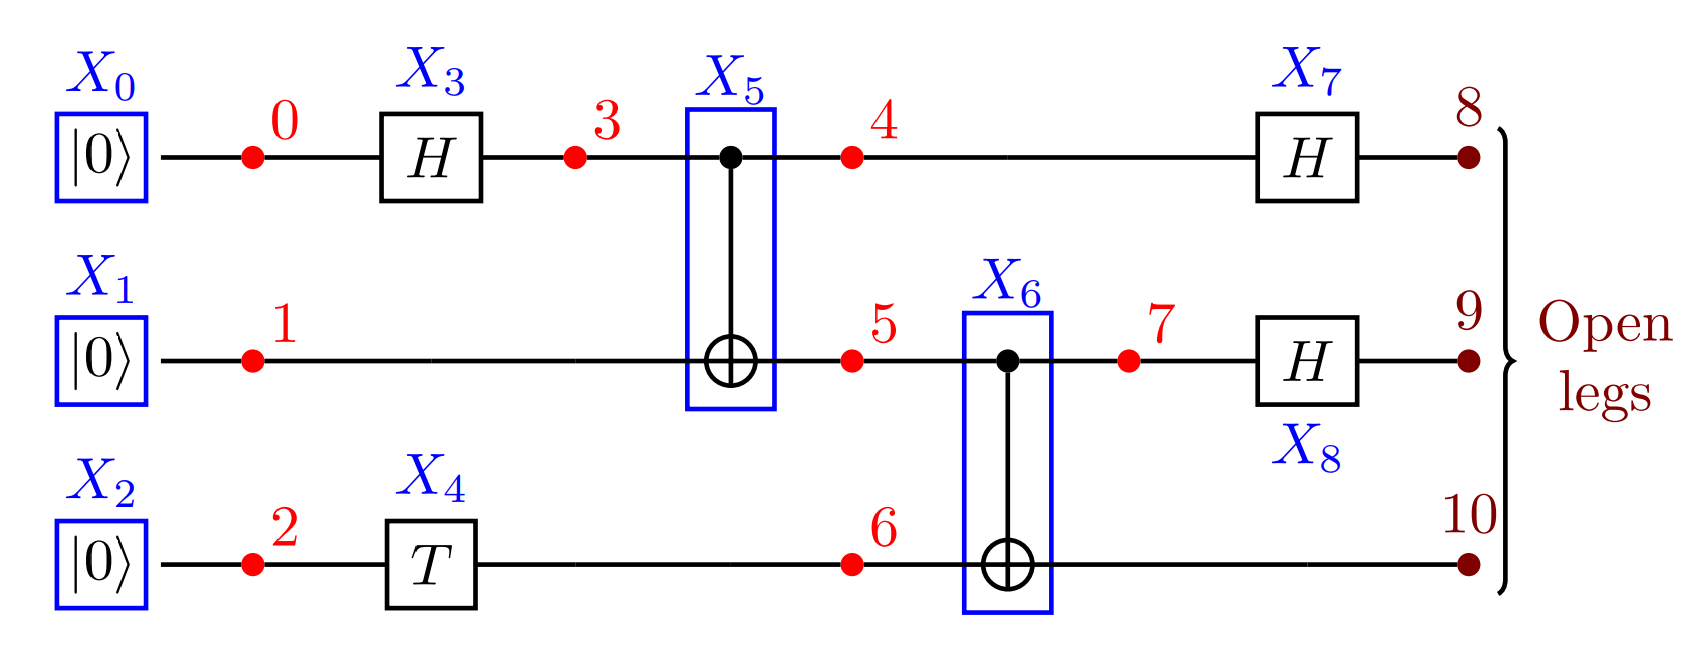
\includegraphics[width=\textwidth]{images/6_3_circ.png}
        \caption{The quantum circuit.}
        \label{6_3_circ}
    \end{subfigure}
    \begin{subfigure}{0.4\textwidth}
        \centering
        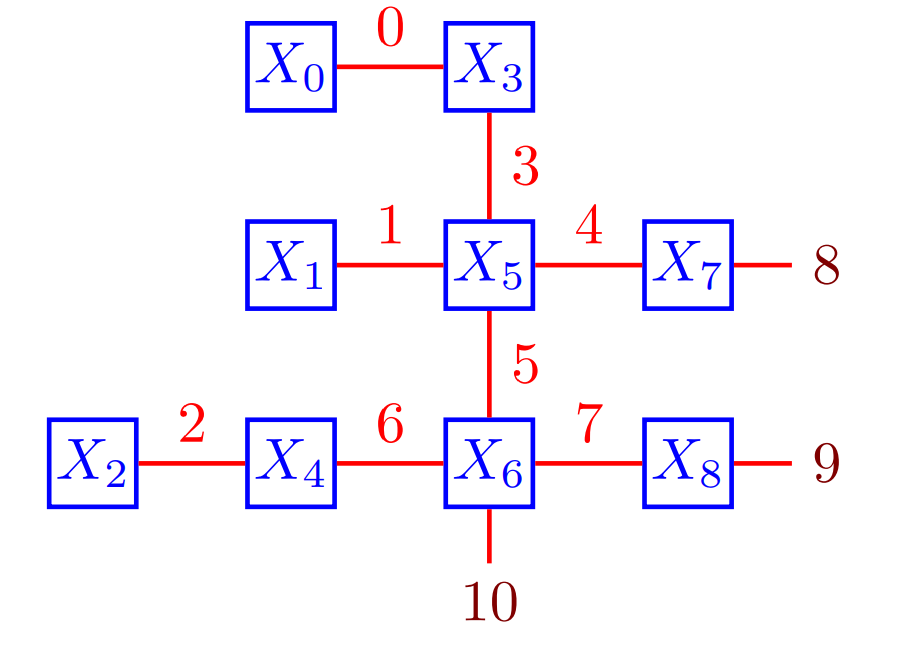
\includegraphics[width=0.9\textwidth]{images/6_3_tn.png}
        \caption{The tensor network.}
        \label{6_3_tn}
    \end{subfigure}
    \caption{An example of the quantum circuit and the corresponding tensor network.}
    \label{fig:6_3_tn_circ}
\end{figure}

Take the Fig.~\ref{fig:6_3_tn_circ} for example, $(X_{0}, \ldots, X_{8})$ are the tensors in this tensor network. We denoted the legs by the~numbers 0--7, and the~open legs by the~numbers 8--10.

A direct application of the tensor approach typically leads to an exponential increase in complexity as the number of qubits and circuit depth grows. This makes simulating large-scale circuits challenging to achieve within a reasonable timeframe. However, when the simulation is performed by calculating only one or a small batch of state amplitudes at the circuit's end, the tensor network's complexity is limited by the size of the largest tensor involved in the contraction process. This size, in turn, grows exponentially with the tree width of the graph corresponding to the tensor network \cite{Markov_2008}.

In \QuPack, we offer an ultra-fast tensor network simulation method for computing single amplitudes and multi-amplitudes \cite{kalachev2022multitensor}, and we also provide circuit sampling simulation capabilities for hundreds of qubits. In addition, we have also implemented quantum noise channels in tensor network simulation, enabling us to simulate the behavior of very large real-world quantum chips.
% \begin{figure}[h]
%   \begin{center}
%     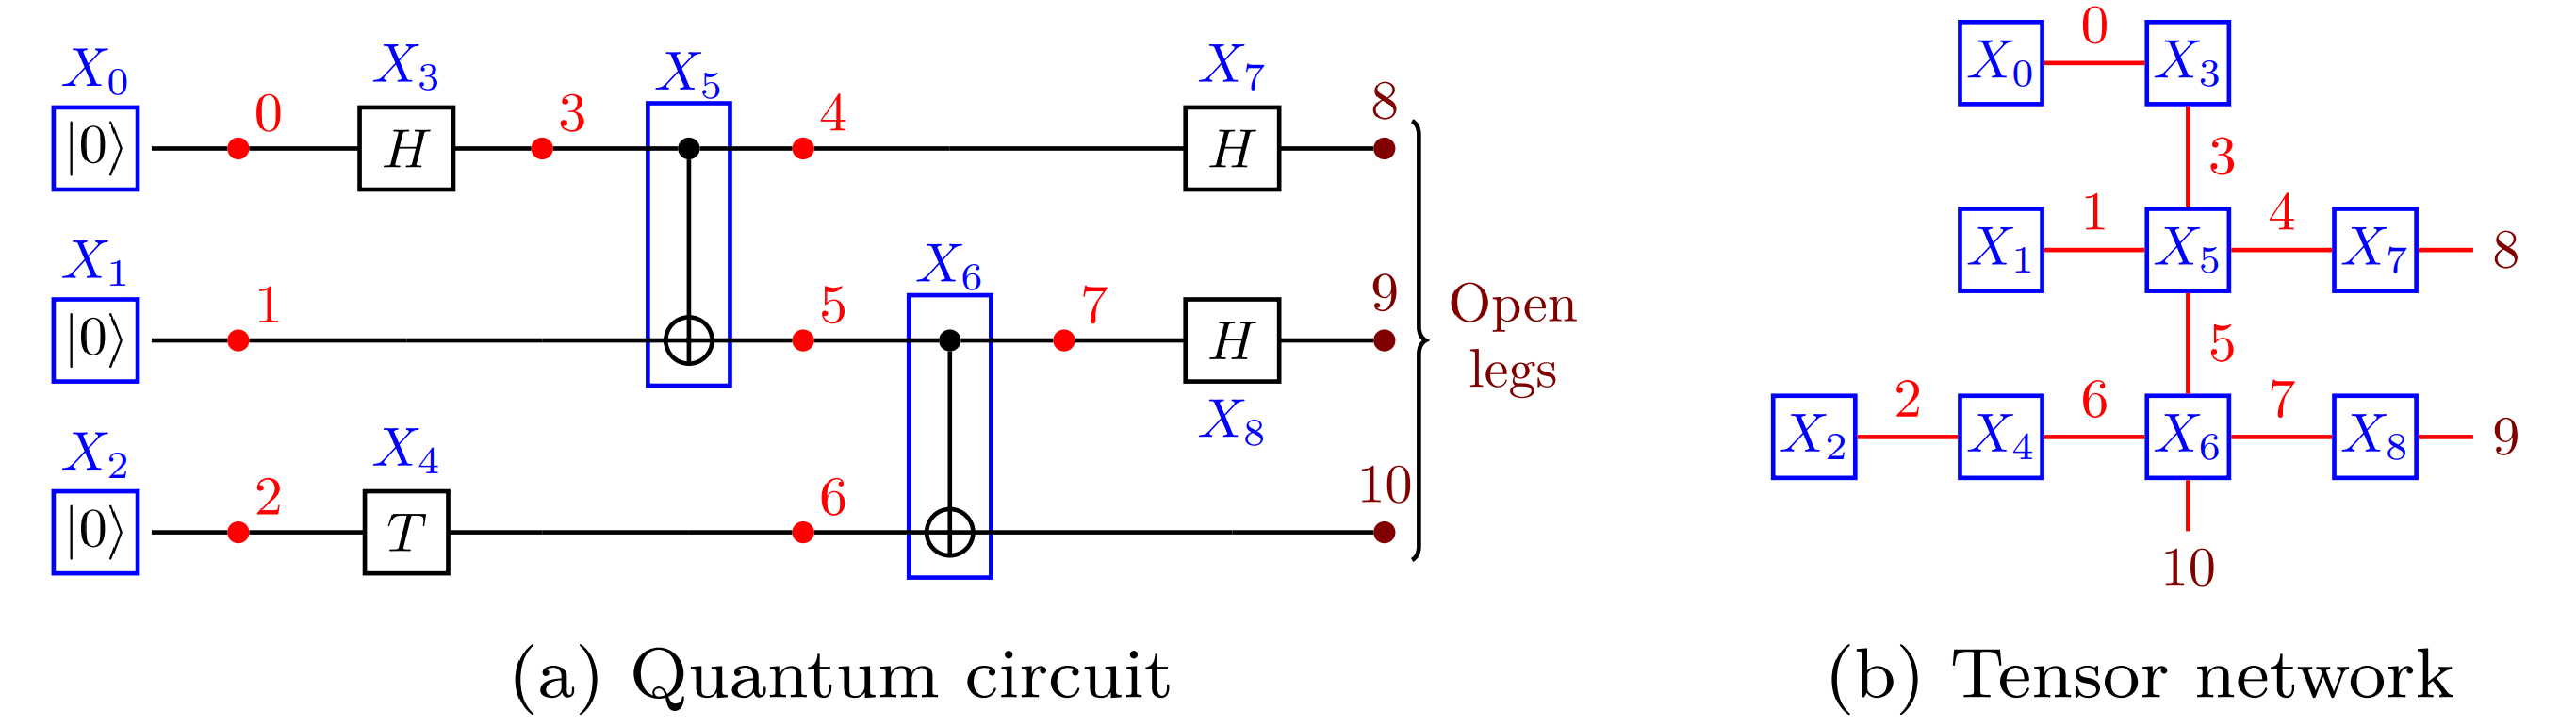
\includegraphics[width=0.9\linewidth]{images/6_3_tn_circ.png}
%   \end{center}
%   \caption{Example for quantum circuit and tensor network.}
%   \label{fig:6_3_tn_circ}
% \end{figure}

\subsubsection{Basic Usage}
In the following, we will provide a detailed explanation of the usage of this Tensor network simulator.
This module supports the following methods: Sampling,  expectation, and amplitudes calculation.

\textit{Sampling and expectation} -- The usage is exactly the same as the method in \MindQuantum. Actually we just wrap the tensor simulator 'MQ\_TNSim' as a backend for \MindQuantum \  simulator so that it supports all the functions as before.
\begin{lstlisting}
from qupack.tensor import MQ_TNSim
sim = Simulator(MQ_TNSim(n_qubits=n_qubits), n_qubits)
res = sim.sampling(circ, shots=shots)
\end{lstlisting}

\textit{Amplitudes calculation} -- The calculation of amplitudes constitutes a specific functionality within the tensor network simulator. While the computation of the full-amplitude obviates the necessity for this functionality due to its inclusion of all amplitudes, amplitude calculation plays a pivotal role in certain processes such as XEB calculation and tasks involving large-scale circuit sampling. Consequently, in this context, the tensor network simulator \code{TNSimulator} is employed exclusively for amplitude calculations.

\begin{lstlisting}
from qupack.tensor import TNSimulator
sim = TNSimulator(circuit_file='data/circuits/simple/circuit_n12_m14_s0_e0_pEFGH.qsim', backend='numpy')  # available backends : numpy, cupy, csim
n = sim.qubit_count
bitstring = [randint(0,1) for i in range(n)]
amp = sim.get_amplitude(bitstring)
\end{lstlisting}

When \code{TNSimulator} is initialized, the following backends can be specified for different tasks:
\begin{itemize}
    \item numpy --- Standard library for tensor operations on CPU. Fastest for simple circuits but very slow in multi-amplitude simulation mode.
    \item cupy --- GPU tensor contraction backend. Good for circuits of intermediate complexity.
    \item csim --- CUDA implementation of simulator. Fastest for long simulations (> 10 seconds), but has sufficient overhead for simpler cases.
\end{itemize}

In addition to single amplitude calculation, it also accommodates multiple amplitudes and batch amplitudes calculations:
\begin{lstlisting}
# batch-amplitudes
amps = sim.get_batch(bitstring, output_idx=[0,1,2])
# multi-amplitudes
amps = sim.get_amplitudes(bitstrings)
\end{lstlisting}

